% !TEX root = ../00_thesis.tex
\section{Implementing the Concepts}
\label{sec:baloo_implementation}

\begin{figure}
	\centering
	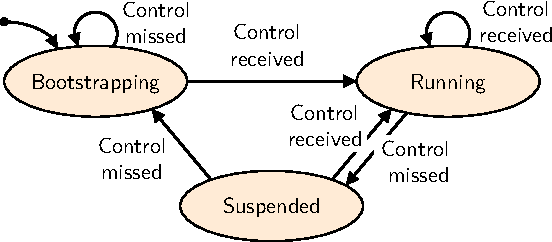
\includegraphics[scale=1]{state-machine}
	\caption{The middleware in \baloo implements a minimal state machine, sufficient to capture the desired behaviour of a node at physical layer.
		\capt{A node either executes normally (\textsl{Running}), stays synchronized but does not participate to the communication rounds (\textsl{Suspended}), or continuously listens for an incoming control packet (\textsl{Bootstrapping}).}}
	\label{fig:state-machine}
\end{figure}

The previous section described the general concepts of \baloo.
% , and discussed how they meet challenges \chal{1}-\chal{3}, presented in the Introduction.
In this section, we present how we implemented these concepts to meet the \feature{Synchronicity} requirement and complete the design of \baloo.

\subsection{Contiki as Operating System}
\label{subsec:contiki}


\baloo relies on the availability of \ST primitives (\eg Glossy~\cite{ferrari2011Glossy}, Chaos~\cite{landsiedel2013Chaos}, \etc). Most openly available primitives use Contiki~\cite{dunkels2004Contiki} as the underlying operating system, which made Contiki an obvious choice to implement \baloo.
We have ported these primitives to the new version of the OS: Contiki-NG~\cite{ContikiNG}.%
\footnote{v4.2, released in November 2018}

Contiki is a cooperative multi-threaded OS, tailored for resource-constrained devices in the Internet of Things.
The middleware layer is implemented as the ``master'' protothread~\cite{dunkels2006Protothreads}, where most of the program is executed. The middleware implements the communication rounds, controls the radio operations, and executes the callback functions in which the network protocol logic is implemented (see \cref{subsec:CB}).


\subsection{Minimal State Machine}
\label{subsec:state-machine}
For generality and simplicity, the middleware implements only a minimal state machine. A node is either in \textsl{Bootstrapping}, \textsl{Suspended}, or \textsl{Running} state.
State transitions result from (un)successful receptions of control packets (see \cref{fig:state-machine}).
When bootstrapping, a node continuously listens for a control packet. In the \textsl{Suspended} state, a node does not participate in the round and will sleep until the next round.

As described in \cref{sec:baloo_overview}, a node may participate in a round (\ie be in the \textsl{Running} state) if and only if it correctly receives the control packet at the beginning of the round.
%
The default behaviour of \baloo is that a node suspends itself if it misses a control packet, and goes back to Bootstrapping if it misses two in a row. A node exits the \textsl{Bootstrapping} state whenever it receives a control packet containing both scheduling and configuration information, \ie when a node knows with certainty how it is expected to operate.
%
If necessary, the network layer protocol can extend this minimal state machine using one of the callback functions (see \cref{subsec:add_func}).

\subsection{Middleware Callback Functions}
\label{subsec:CB}

\baloo uses callback functions to implement the network layer protocol logic. This is how the network layer interacts with the middleware at runtime (\feature{Usability}).
%
There are five different callbacks, which have specific purposes and are executed by the middleware at precise points in time, as illustrated in \cref{fig:callbacks}.

\begin{functions}

	\item[on\_control\_slot\_post()]~\newline
	is executed at the end of the control slot.
	It is used to process the received control information and prepare for the round.

	\item[on\_slot\_pre()]~\newline
	is executed before each data slot.
	It is used to pass the payload to send to the middleware, if any.

	\item[on\_slot\_post()]~\newline
	is executed at the end of each data slot.
	It is used to process the received payload, if any.

	\pagebreak
	\item[on\_round\_finished()]~\\
	is executed at the end of the round.
	It is used to do more time consuming state management or data processing.

	\item[on\_bootstrap\_timeout()]~\newline
	is executed when a node fails to bootstrap (\ie it has listened for some time without receiving any control packet).
	This callback allows nodes to go to sleep and retry bootstrapping later, in order to save energy.

\end{functions}

These callback functions are also used to implement more advanced features of \baloo (\eg skipping or repeating a slot), which are briefly presented in \cref{sec:adv_features}.

\afterpage{
	\begin{landscape}
		\begin{figure*}
			\centering
			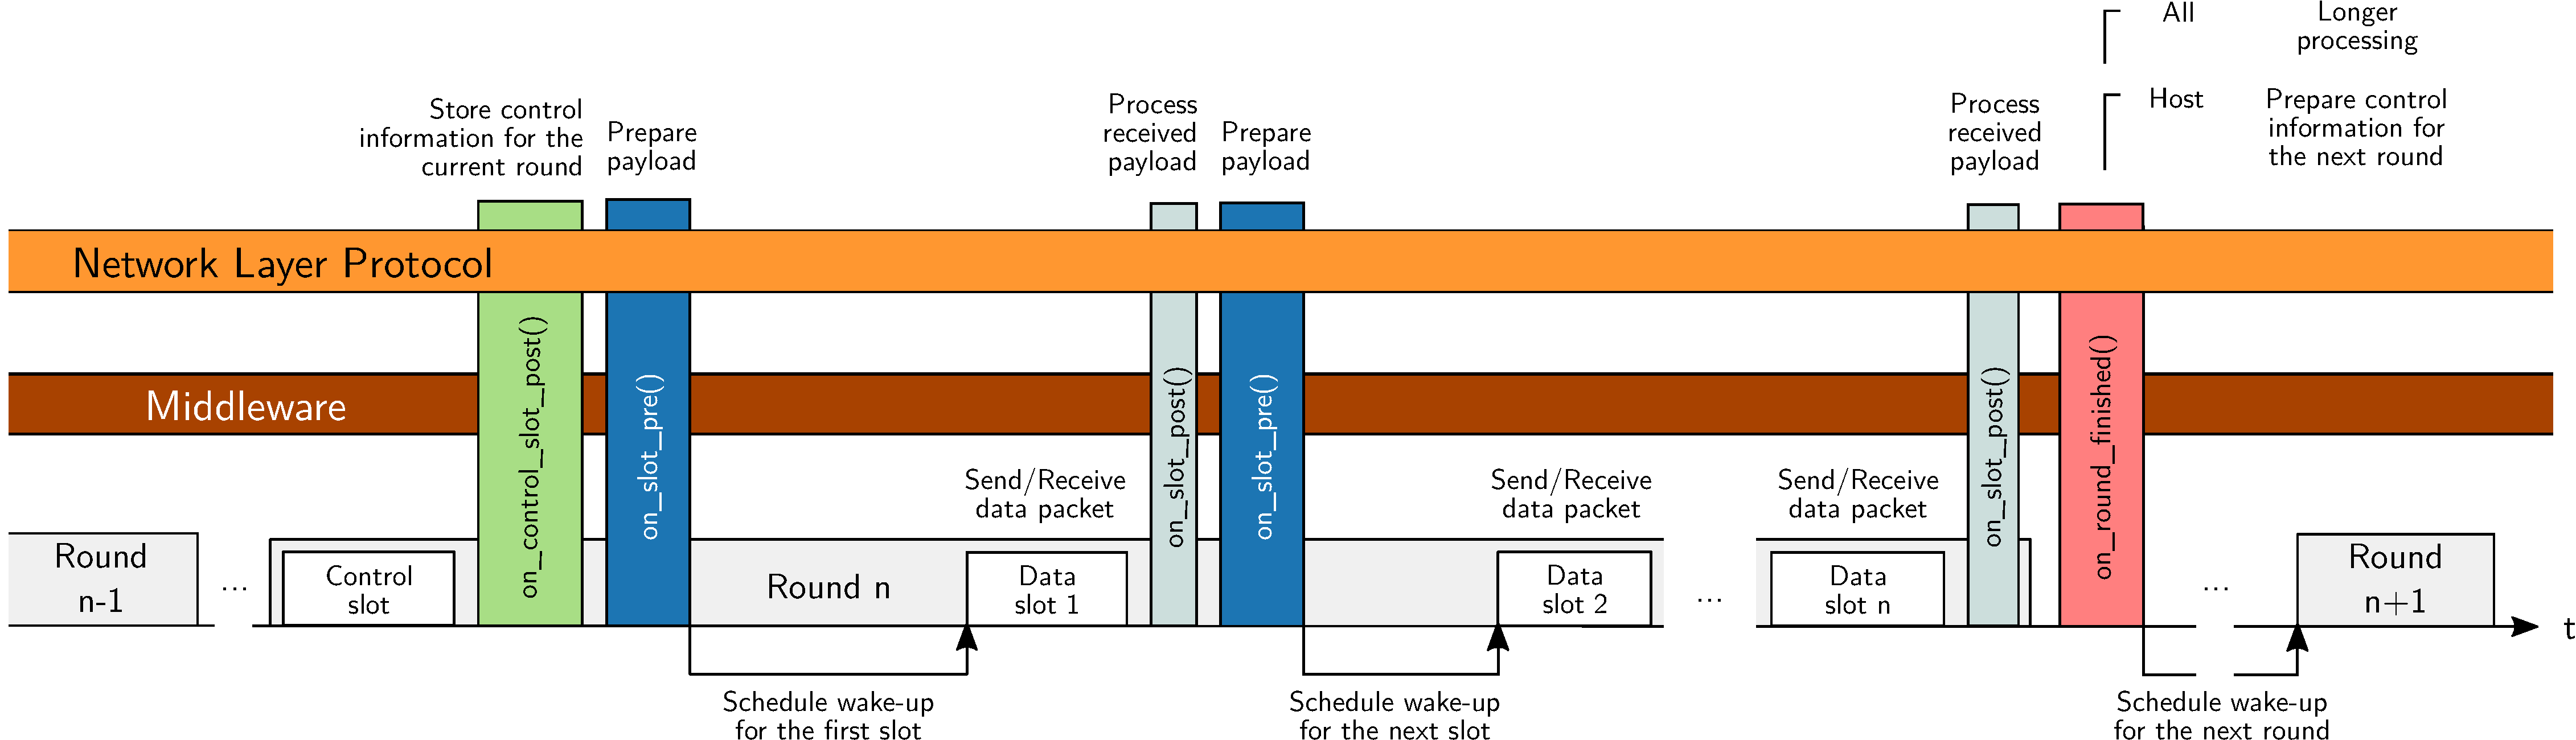
\includegraphics[width = \linewidth]{callbacks}
			\caption{The protocol logic, \ie the handling of application payloads and the definition of the desired control parameters, is implemented in callback functions. These callbacks are triggered by the middleware before and after each slot and at the end of a round.
				The middleware schedules the wake-up of the radio core and executes the \ST primitives.}
			\label{fig:callbacks}
		\end{figure*}
	\end{landscape}
}


\subsection{Achieving Timeliness of Execution}
\label{subsec:timeliness}

The callback functions enable flexible interactions between the network layer and the middleware. While this is key to address \feature{Usability} and \feature{Generality}, it also inherently couples the two software components, thus challenging the timely execution of the middleware and compromising \feature{Synchronicity}.

Indeed, the callbacks execute between communication slots or between rounds (see \cref{fig:callbacks}), which must start synchronously on all nodes to permit successful \ST.
The middleware could interrupt an overrunning callback to ensure synchronicity, but that is not desirable. In general, an interrupted callback would have to be considered as a failure by the network layer; then successful \ST at the lower layer would not really matter anyway.

To mitigate this problem, the middleware \textsl{monitors} the execution time of the callbacks. If a callback overruns and the middleware cannot guarantee the timely execution of the next slot, this slot is skipped (\ie the node does not participate at all in this slot) and a notification event is sent to the network layer.

With this approach, \baloo can guarantee to respect the timing requirement for \ST \textit{under the condition that the callbacks have enough time to complete their execution}.%
\footnote{This default strategy may lead to a starvation problem if a callback ``never'' returns, \eg if it relies on another software sitting at higher layers. One advanced feature lets the middleware interrupt overrunning callbacks (see \cref{subsec:add_func}).}
To satisfy this condition, the available time between slots for the execution of the callbacks is controlled by a dedicated configuration parameter: the \textsl{gap time}.
Since callbacks implement the network layer protocol logic, it can only be the responsibility of the network designer to set suitable gap times such that the \feature{Synchronicity} requirement is met.
Guidelines for setting such parameters (and in general: how-to use \baloo) are part of the online documentation~(\cref{append:baloo_artifacts}).
\subsection{Supporting Multiple \ST Primitives}
\label{subsec:multi-ST-primitives}

Compared to previously proposed low-power network stacks, one key difference of \baloo is that it flexibly supports multiple \ST primitives (\feature{Versatility}).
This is difficult given the nature of \ST, which requires tight timing of radio events (from sub-\us to tens of \us depending on the primitive~\cite{yuan2013LetTalkTogether}).

In practice, achieving such synchronization requires a direct monitoring of hardware timers and a custom implementation of the associated Interrupt Service Routines (ISR) for each \ST primitive executed by the middleware in \baloo.
However, there cannot be multiple implementation of the same ISR. Thus, supporting multiple \ST primitives in the same stack requires to extract the interrupt management from the \ST code, which becomes a shared software component between different primitives.

Technically, we implemented this using a renaming trick. Indeed, each \ST primitive has its own ISR implementation for the radio timer, but \baloo never uses more than one \ST primitive at the same time (\ie one per data slot). The middleware must only execute the instructions of the ISR from the currently running primitive.
Thus, we can encapsulate the ISR of each primitive into a dedicated (\ie unique)  function and implement the radio timer ISR as a simple ``switch'' function. A global variable keeps track of the currently running primitive; whenever the radio timer fires, the corresponding primitive ``ISR function'' is executed.

The only difference with the original primitives' implementation is an additional software delay between the radio interrupt and the execution of the ISR's instructions (the few ticks of delay to execute the switch).
This adds a negligible synchronization error due to differences in clock speed across different nodes.%
\footnote{%
	Assuming an absolute clock drift of 100\ppm between two nodes (which is pessimistic), the error introduced is $\sim 0.24$ picosecond per tick of delay.
	}

Using this approach, \baloo currently supports two \ST primitives, Glossy~\cite{ferrari2011Glossy} and Chaos~\cite{landsiedel2013Chaos}, as well as a classical strobing communication primitive: one node transmits its packet, multiple times, while all other nodes only listen.
Practically, there is no limitation on the number of primitives that \baloo can support, apart from the available memory.
